\documentclass[a4paper,10pt,notitlepage]{scrreprt}

\usepackage[T1]{fontenc}
\usepackage[english]{babel}
\usepackage[utf8x]{inputenc}
\usepackage{setspace}
\usepackage{subfig}
\usepackage{textcomp}
\usepackage{graphicx}
\usepackage{fixltx2e}
\usepackage{multirow}
\usepackage{array}
\usepackage{amssymb}
\usepackage{amsmath}
\usepackage{subfig}
\usepackage{nomencl}
\usepackage[pdfborder={0 0 0}]{hyperref}
\usepackage{natbib}
% \usepackage{makeidx}
\usepackage{nicefrac}
\usepackage{bbold}

\captionsetup{labelfont=footnotesize,textfont=footnotesize}

\newcolumntype{x}[1]{>{\begin{flushleft}$}p{#1}<{$\end{flushleft}}}
\newcolumntype{y}[1]{>{\begin{center}$}p{#1}<{$\end{center}}}
\newcolumntype{z}[1]{>{\begin{flushright}$}p{#1}<{$\end{flushright}}}
\newcolumntype{m}{>{$}l<{$}}
\newcolumntype{n}{>{$}c<{$}}
\newcolumntype{o}{>{$}r<{$}}

% Title Page
\title{Scientific Visualization\\Project I}
\author{Milian Wolff}


\begin{document}
\maketitle

\begin{abstract}
In the first project for the scientific visualization class by Eugene Zhang I
got some first hand experience in 3D visualization algorithms, Java programming
and JavaView. While the former was very interesting and gave many opportunities
to play with parameters, models and algorithms, the latter two I could have
done without. Especially the severe lack of up-to-date documentation for the
required beta release of JavaView along with its horrible API made me waste a
lot of time.
\end{abstract}

\begingroup
\let\clearpage\relax

\tableofcontents
\endgroup

\chapter{Euler Characteristics}

The relationship between the euler characteristic $V-E+F$ and the number of
handles turns out to be

\begin{equation}
 V-E+F = 2-2H .
 \label{eq:handle-euler}
\end{equation}

This is in so far intuitive as $2$ is the euler characteristic of a sphere, and
$0$ that of a torus. Now everytime we add another handle, we can say we add a
torus - and hence decrease the euler characteristic by two.

The code for these results can be found in the class \texttt{Ex1\_1}. When
executed, the user can select an \texttt{*.obj} file and the program will
show it's euler characteristic as computed by JavaView's
\texttt{PgPointSet::getEulerCharacteristic()} method. It then continues to
iterate over all sibling files with the \texttt{*.obj} extension and repeats the
procedure.

\section{Sphere}

The sphere has no handles, as can be seen in fig. \ref{fig:sphere}. As such its
euler characteristic is of course $2$.

\begin{figure}
  \centering

  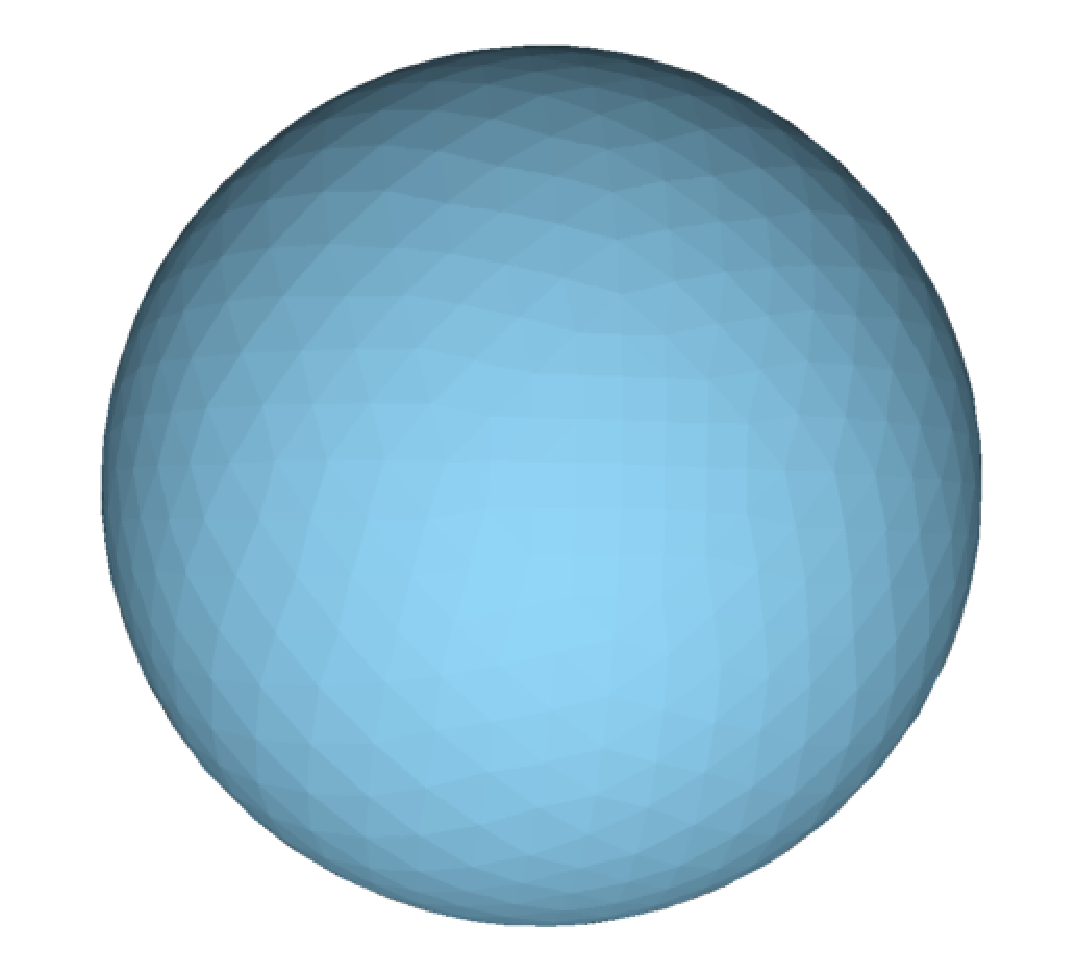
\includegraphics[scale=0.5]{sphere.eps}

  \caption{Sphere}
  \label{fig:sphere}
\end{figure}

\section{Torus}

The torus has a single handle and hence an euler characteristic of $0$. See
also fig. \ref{fig:torus}.

\begin{figure}
  \centering

  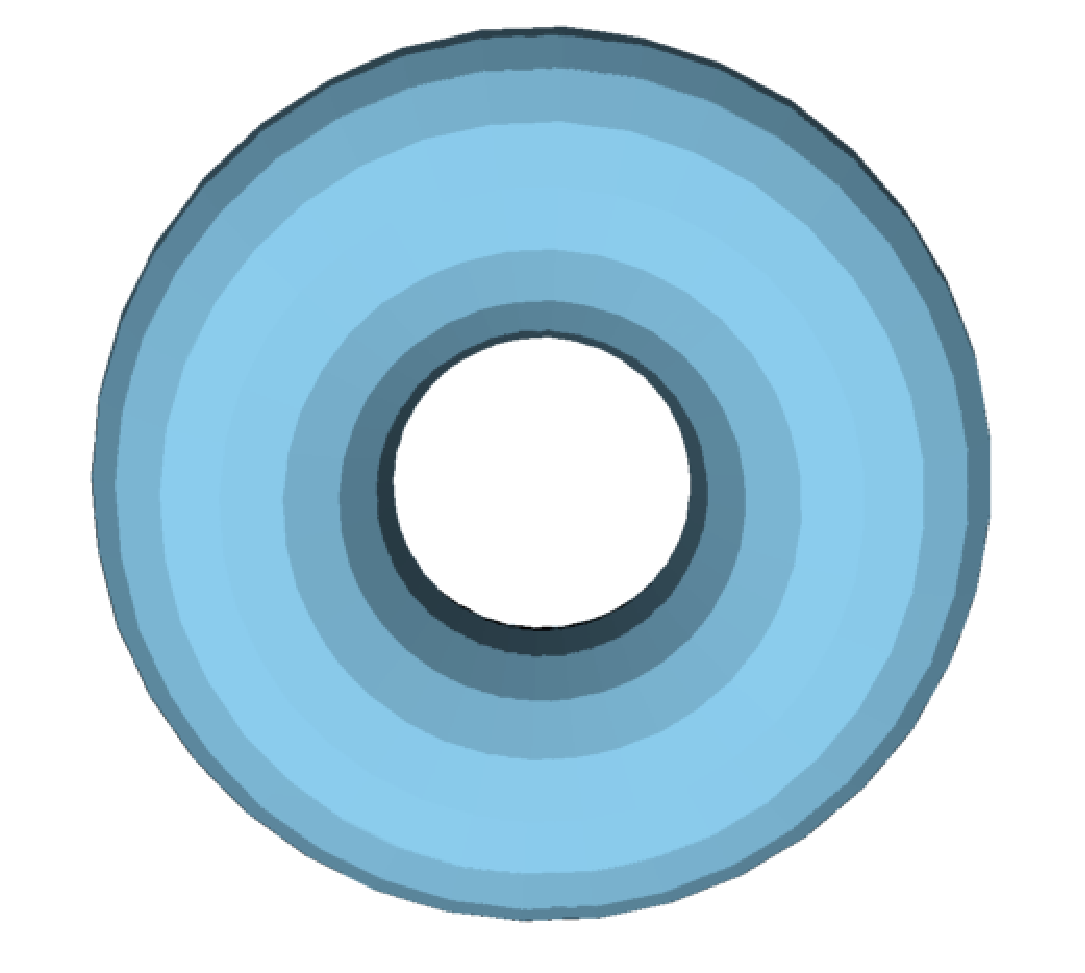
\includegraphics[scale=0.5]{torus.eps}

  \caption{Torus}
  \label{fig:torus}
\end{figure}

\section{Bunny}

The bunny as seen in fig \ref{fig:bunny} has no handles and is thus
topologically equivalent to the sphere with an euler characteristic of $2$.

\begin{figure}
  \centering

  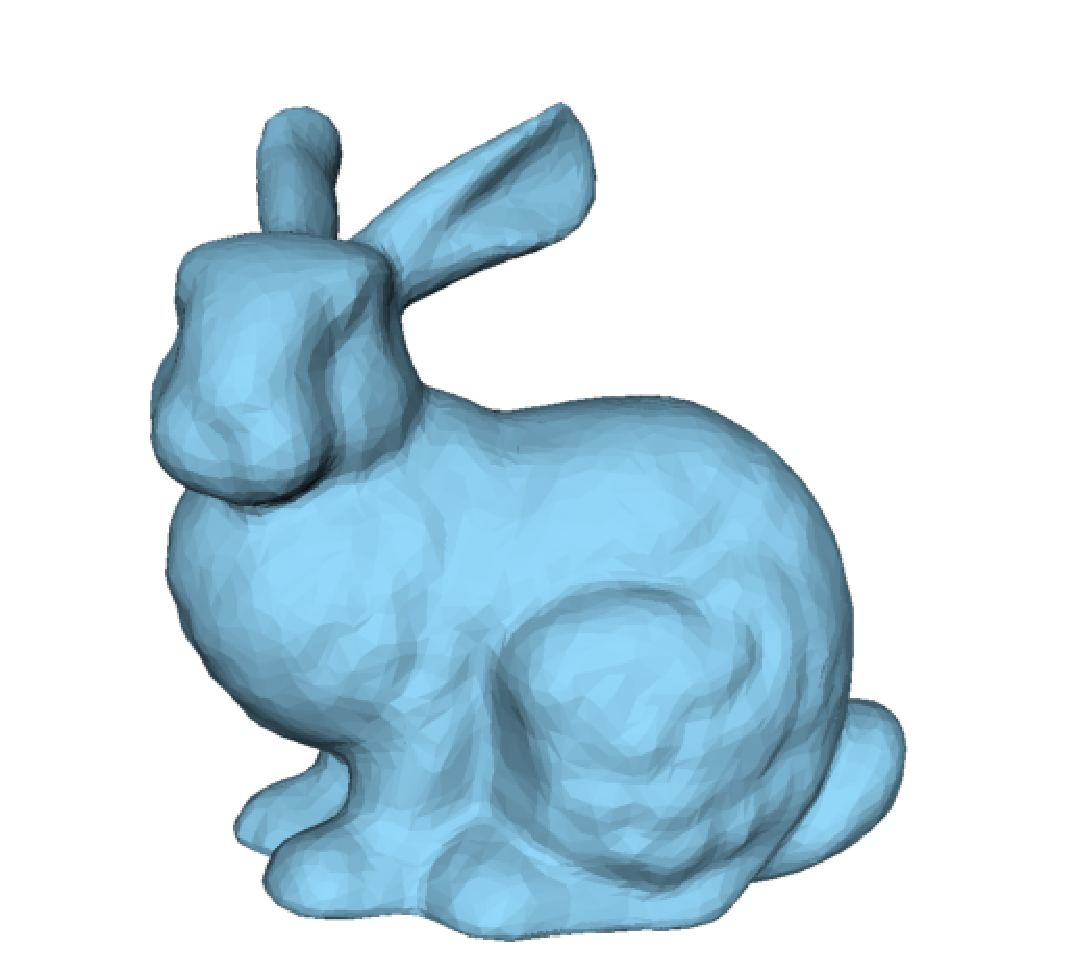
\includegraphics[scale=0.5]{bunny.eps}

  \caption{Bunny}
  \label{fig:bunny}
\end{figure}

\section{Hand}

The hand I first suspected to be handle-free. But JavaView calculated an euler
characteristic of $0$, which made me look for a handle. And indeed, there is a
small hole between index and middle finger, which can be seen in fig.
\ref{fig:hand}.

\begin{figure}
  \centering

  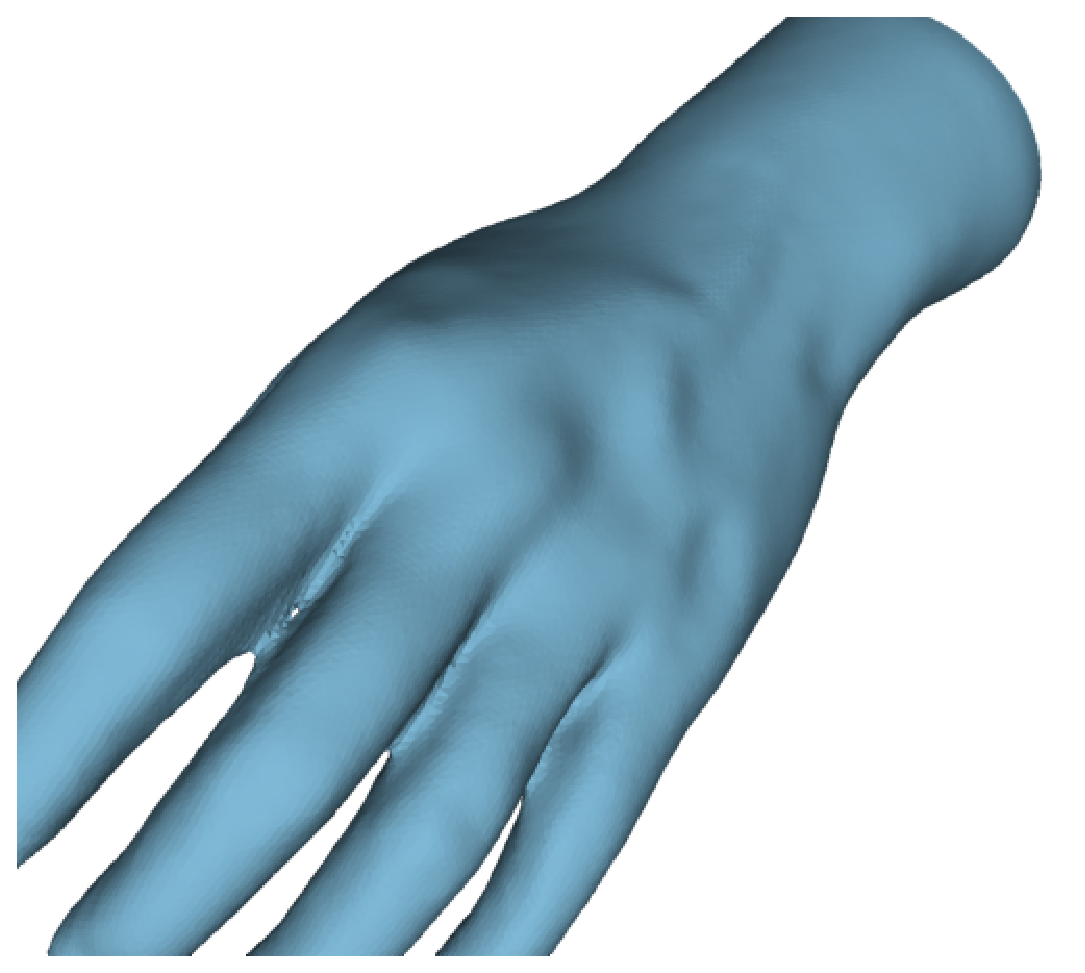
\includegraphics[scale=0.5]{hand.eps}

  \caption{Hand}
  \label{fig:hand}
\end{figure}

\section{Feline}

The feline has two handles at its tail, which is equivalent to an euler
characteristic of $-2$. See also fig. \ref{fig:feline}.

\begin{figure}
  \centering

  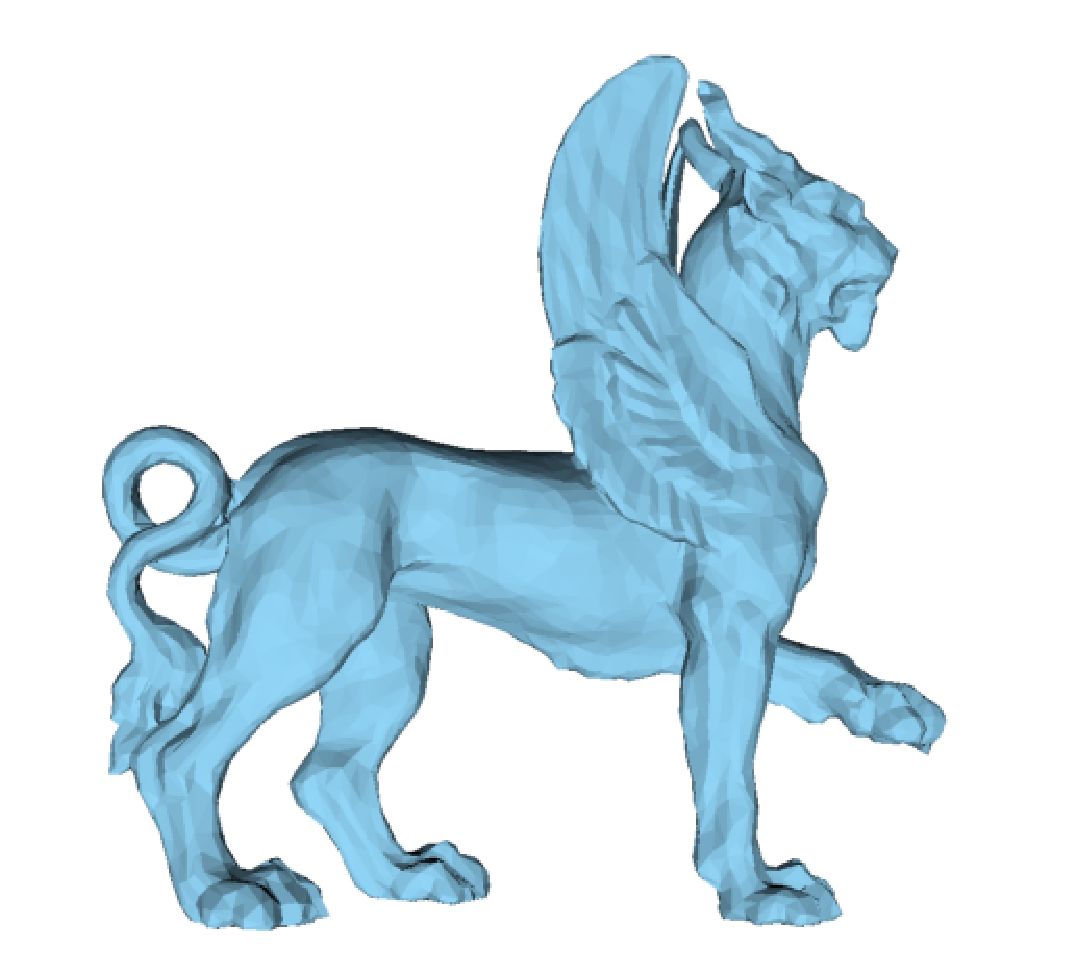
\includegraphics[scale=0.5]{feline.eps}

  \caption{Feline}
  \label{fig:feline}
\end{figure}

\section{Dragon}

The dragon's tail creates a handle near its end. As such it has an euler
characteristic of $0$ and is topologically equivalent to a torus. See also fig.
\ref{fig:dragon}.

\begin{figure}
  \centering

  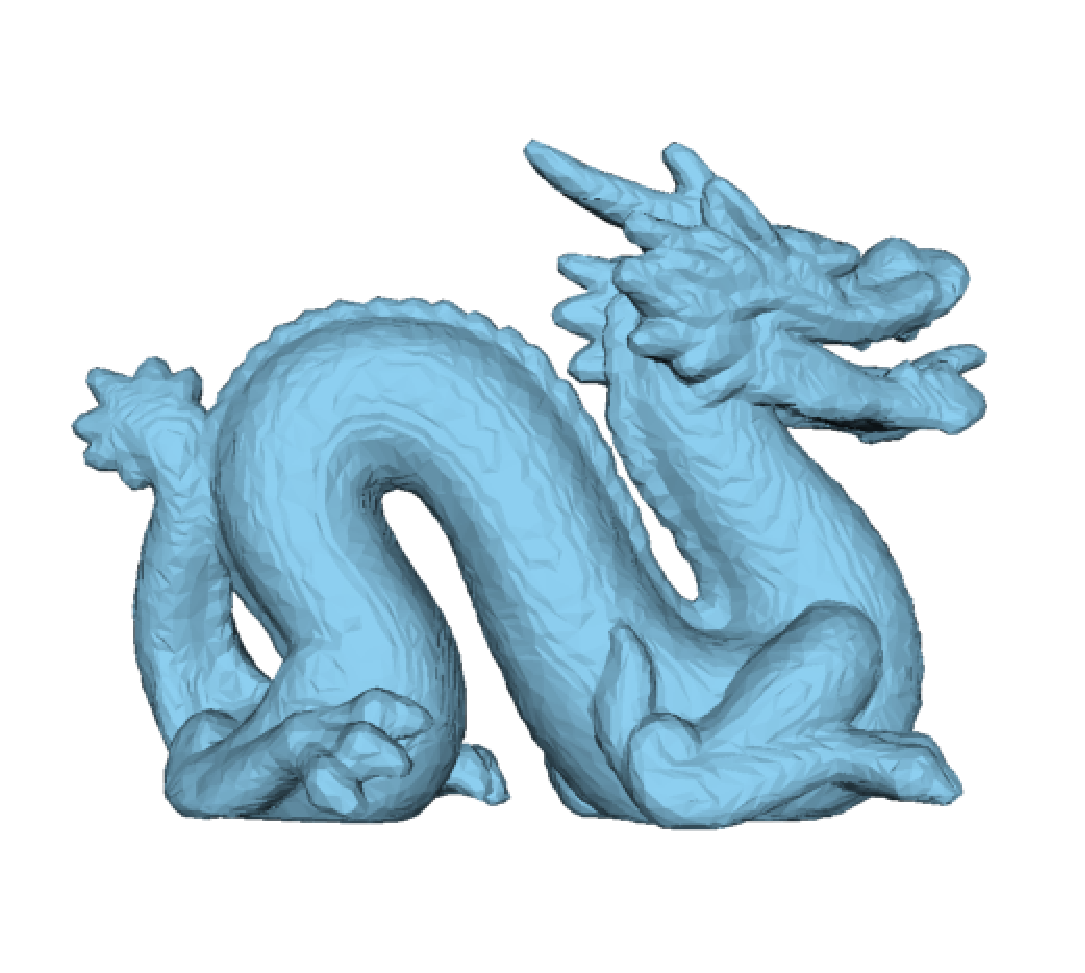
\includegraphics[scale=0.5]{dragon.eps}

  \caption{Dragon}
  \label{fig:dragon}
\end{figure}

\section{Buddha}

The buddha has the most handles of the objects provided. Its euler
characteristic is $-10$, and as such we should find six handles in total. Five
of them are easily visible in fig. \ref{fig:buddha1} while the last one should
be seen from the rotated view in fig. \ref{fig:buddha2}.

\begin{figure}
  \centering

  \subfloat{\label{fig:buddha1}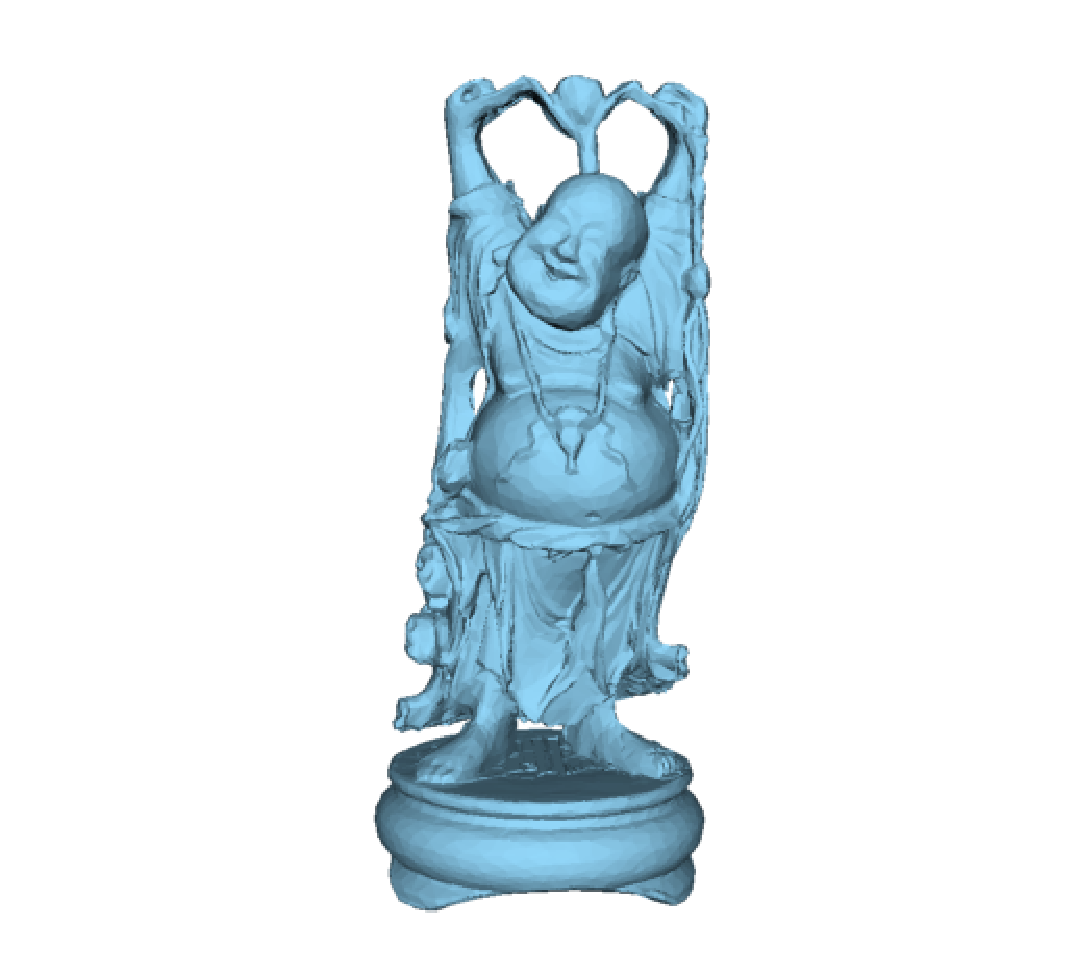
\includegraphics[scale=0.4]{budda.eps}}
  \subfloat{\label{fig:buddha2}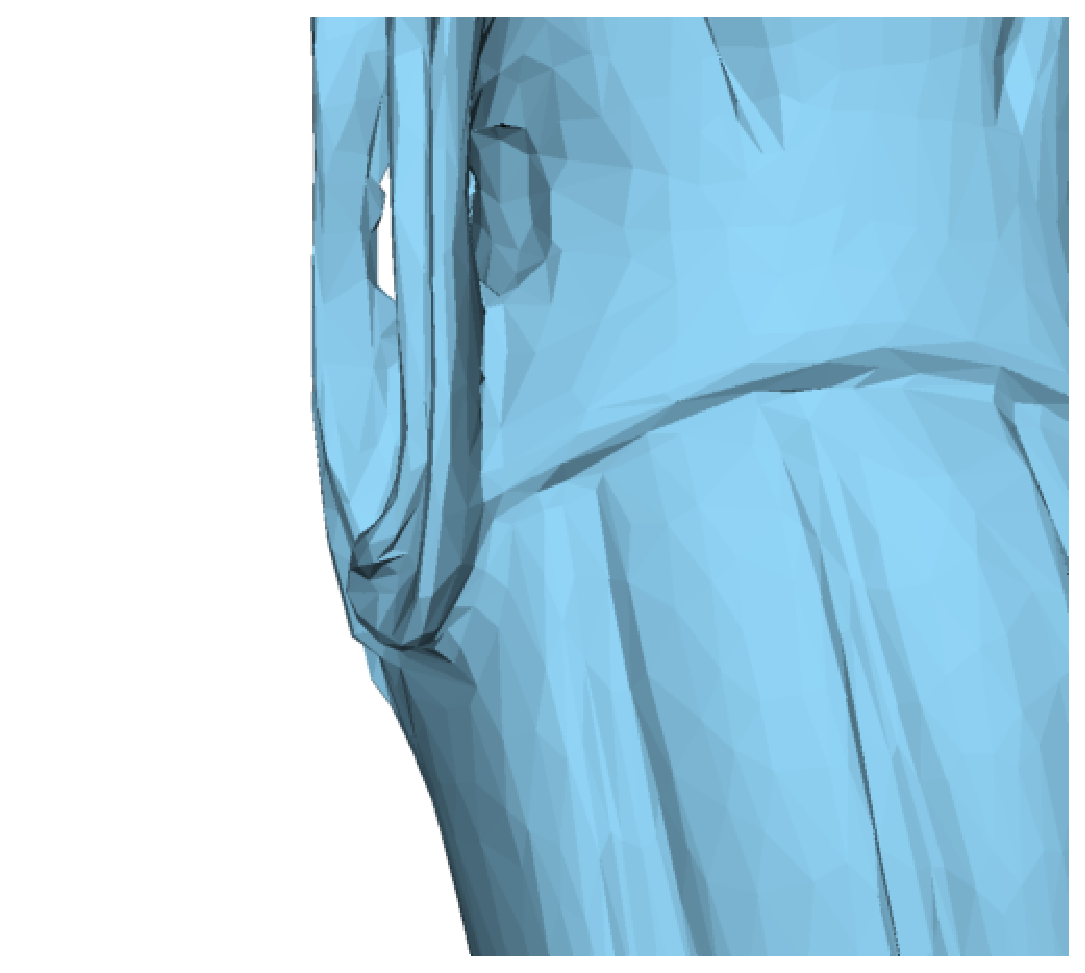
\includegraphics[scale=0.4]{budda2.eps}}

  \caption{Buddha}
\end{figure}

\chapter{Mesh Coloring}

\section{Normal Mapping}

This exercise was straight forward to solve. One just iterates over the
polygons, or ``elements'' in JavaViews terminology, and assigns a color
following the equation as given on the exercise sheet:

\begin{equation}
  R = |N_x|, G = |N_y|, B = |N_z|
 \label{eq:normal-mapping}
\end{equation}

\texttt{Java.awt.Color} comes with a constructor taking three \texttt{float}
arguments. Alternatively we would multiply the absolute value with $255$ and
round off, to get an integer RGB color component value.

The results can be seen in fig. \ref{fig:bunny-normal},
\ref{fig:feline-normal}, \ref{fig:buddha-normal} and \ref{fig:dragon-normal},
and the source code is located in \texttt{Ex1\_2::setNormalMappingColors()}.

\section{3D Checkerboard}

Again, the solution to this exercise was not difficult to program. Again we map
the RGB values to $8$-bit integer values, just set the vertex colors this time.
The elements are then colored by
calling $PgElementSet::showElementFromVertexColors(true)$ on the selected
geometry.

The results can be seen in fig. \ref{fig:bunny-checker},
\ref{fig:feline-checker}, \ref{fig:buddha-checker} and
\ref{fig:dragon-checker},
and the source code is located in \texttt{Ex1\_2::set3DCheckerboardColors()}
and \texttt{Ex1\_2::f()}, while the latter combines two steps from the exercise
sheet, namely the devision by $L$ followed by flooring the result and the
computation denoted by $f(n)$ on the exercise sheet.

Problems with this algorithm are the jagged edges of the single checkerboard
tiles. Especially for lower $L$ this gets worse, as can be seen in e.q. fig.
\ref{fig:dragon-checker}. This problem gets even more prominent when applying
the colorization algorithm to an Icosahedron, as seen in fig.
\ref{fig:icosahedron-checker1} and \ref{fig:icosahedron-checker2}. The reason
for both is the relatively low number of vertices compared to the size of the
polygons. If we would remesh the objects and add more points, the checkerboard
algorithm should work better again.



\begin{figure}
  \centering

  \subfloat[normal mapping]{
    \label{fig:bunny-normal}
    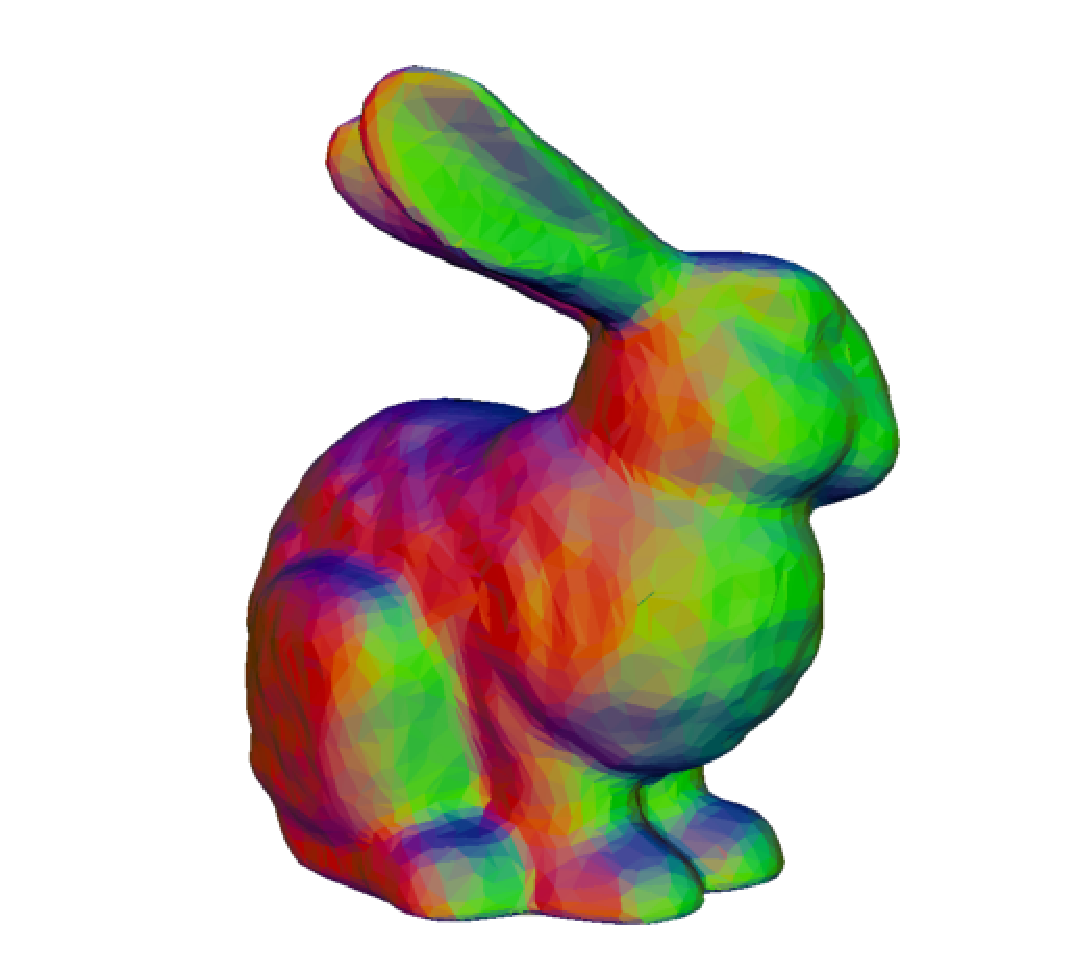
\includegraphics[scale=0.4]{bunny-normal.eps}}
  \subfloat[checker board, $L = 1.0$]{
    \label{fig:bunny-checker}
    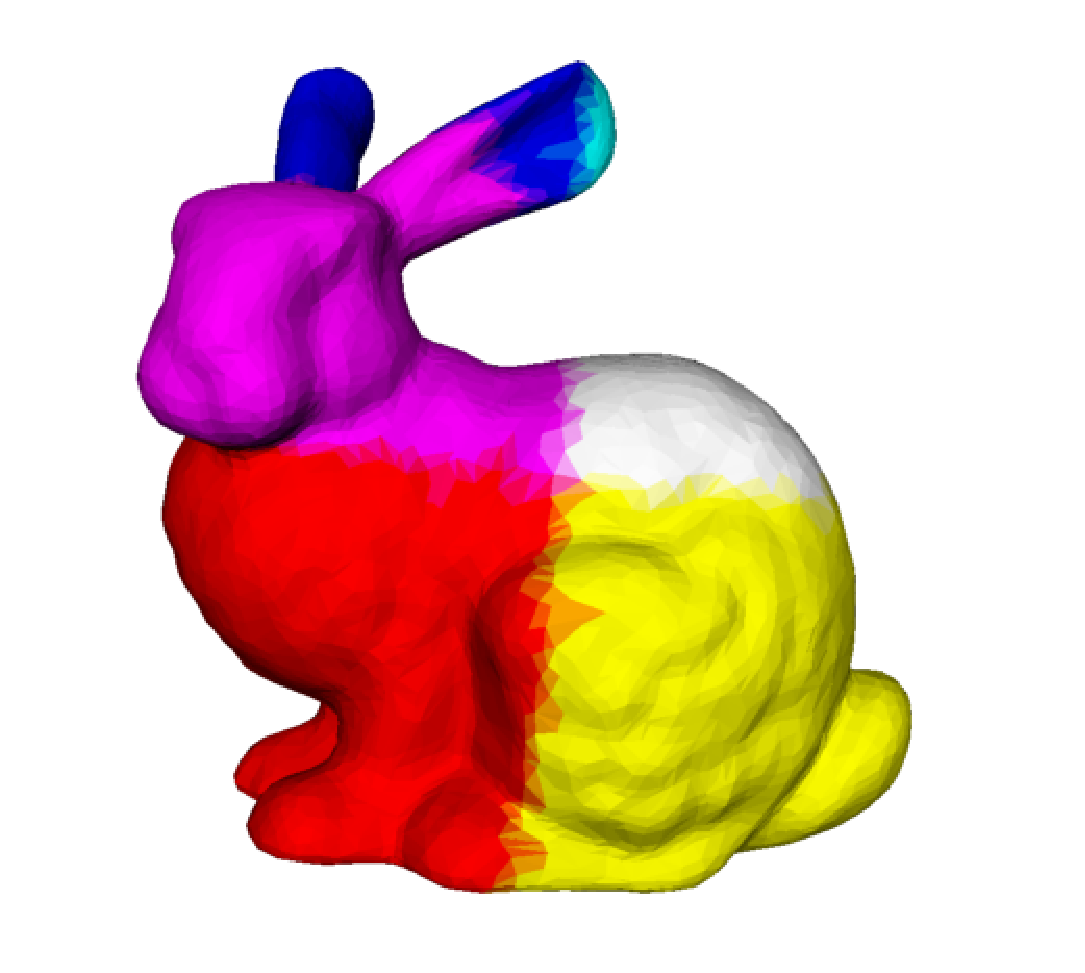
\includegraphics[scale=0.4]{bunny-checker-l1.eps}}

  \caption{Bunny}
\end{figure}

\begin{figure}
  \centering

  \subfloat[normal mapping]{
    \label{fig:feline-normal}
    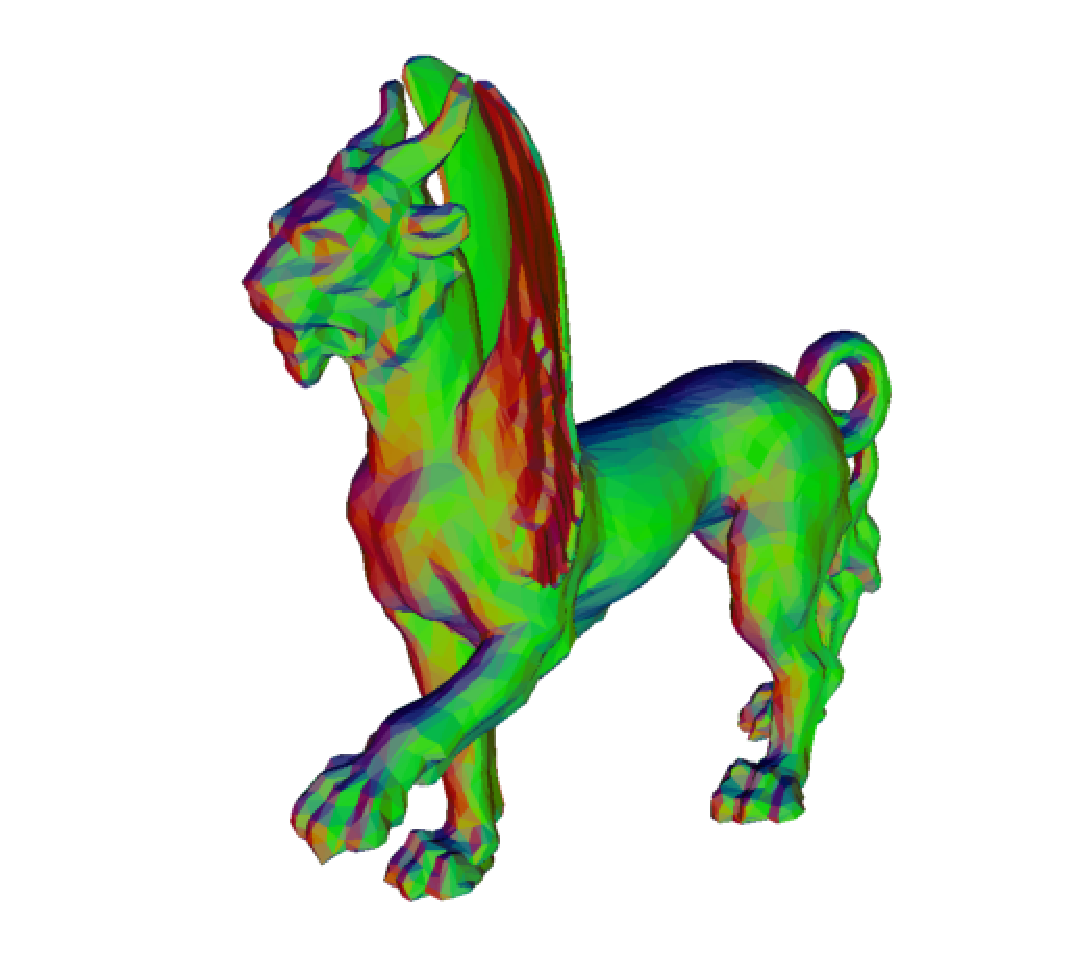
\includegraphics[scale=0.4]{feline-normal.eps}}
  \subfloat[checker board, $L = 0.5$]{
    \label{fig:feline-checker}
    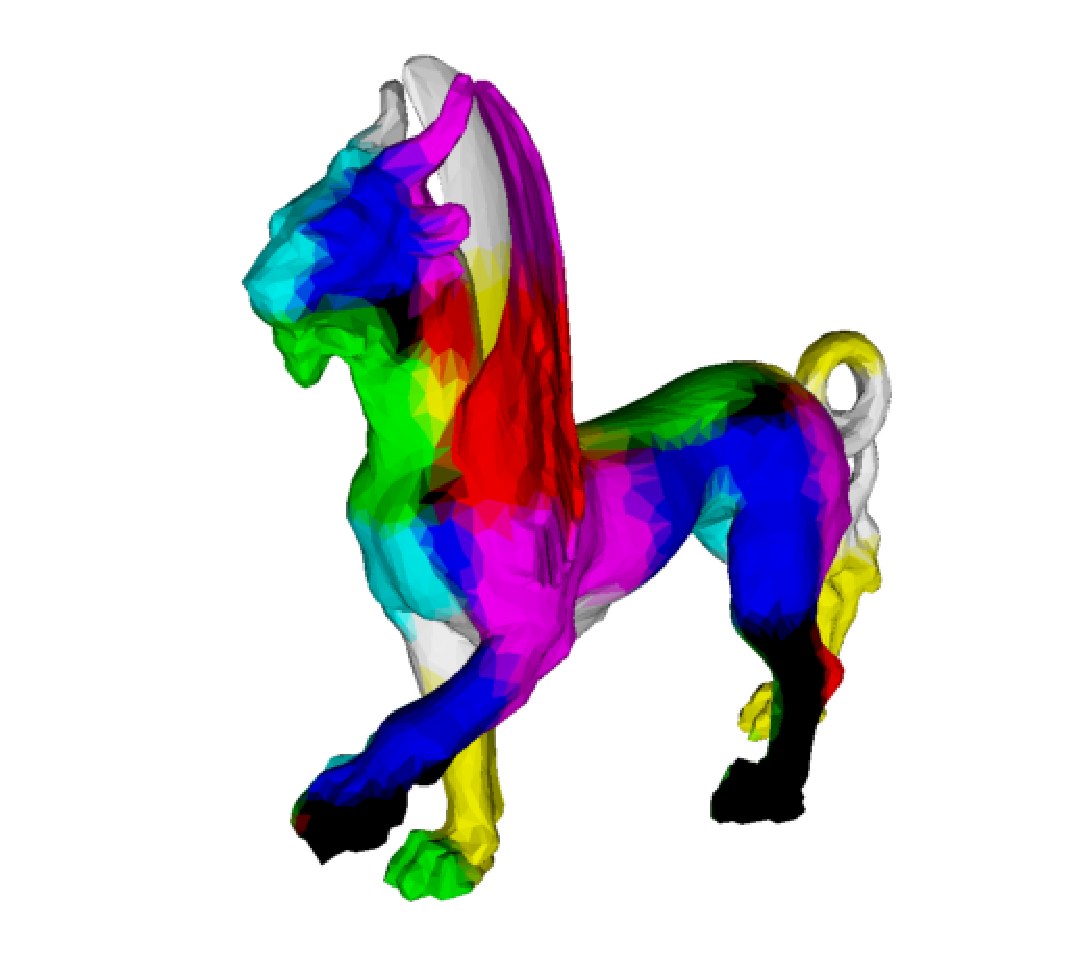
\includegraphics[scale=0.4]{feline-checker-l05.eps}}

  \caption{Feline}
\end{figure}

\begin{figure}
  \centering

  \subfloat[normal mapping]{
    \label{fig:buddha-normal}
    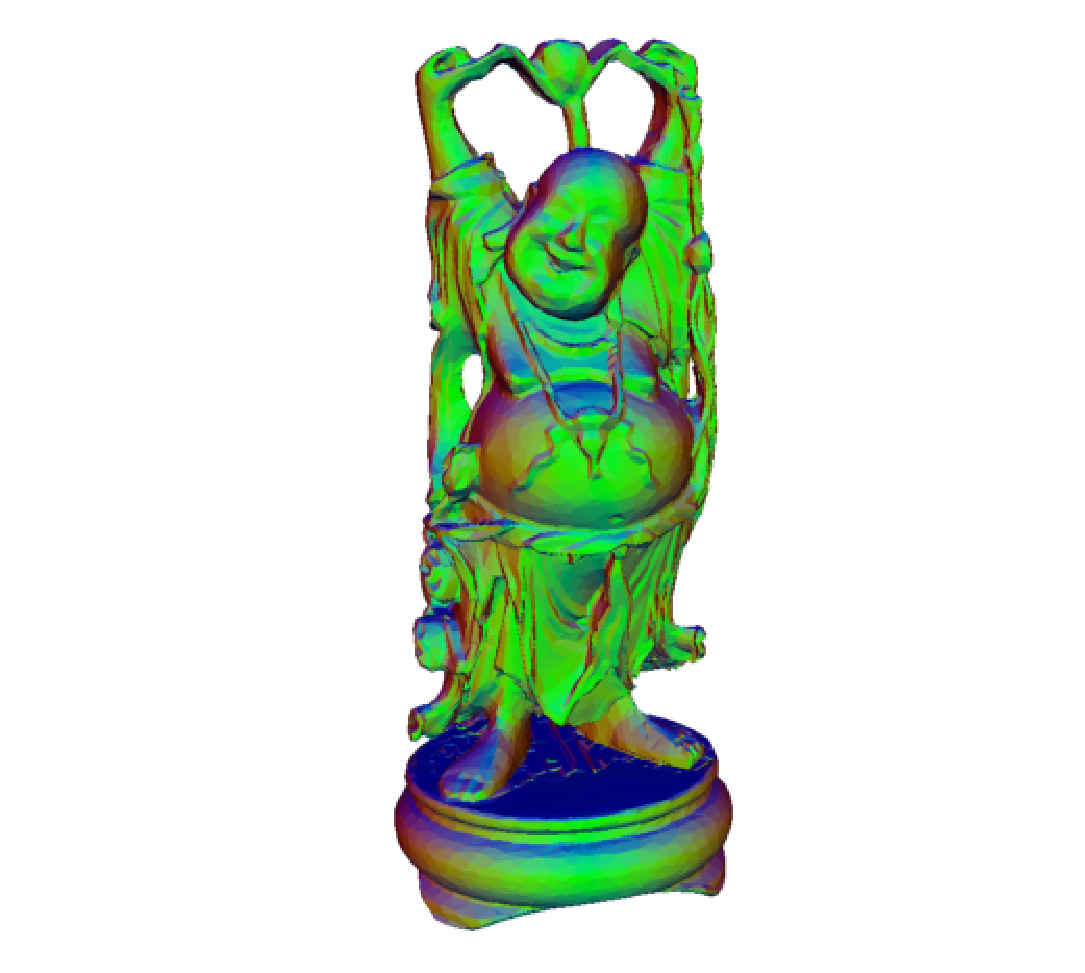
\includegraphics[scale=0.4]{buddha-normal.eps}}
  \subfloat[checker board, $L = 0.25$]{
    \label{fig:buddha-checker}
    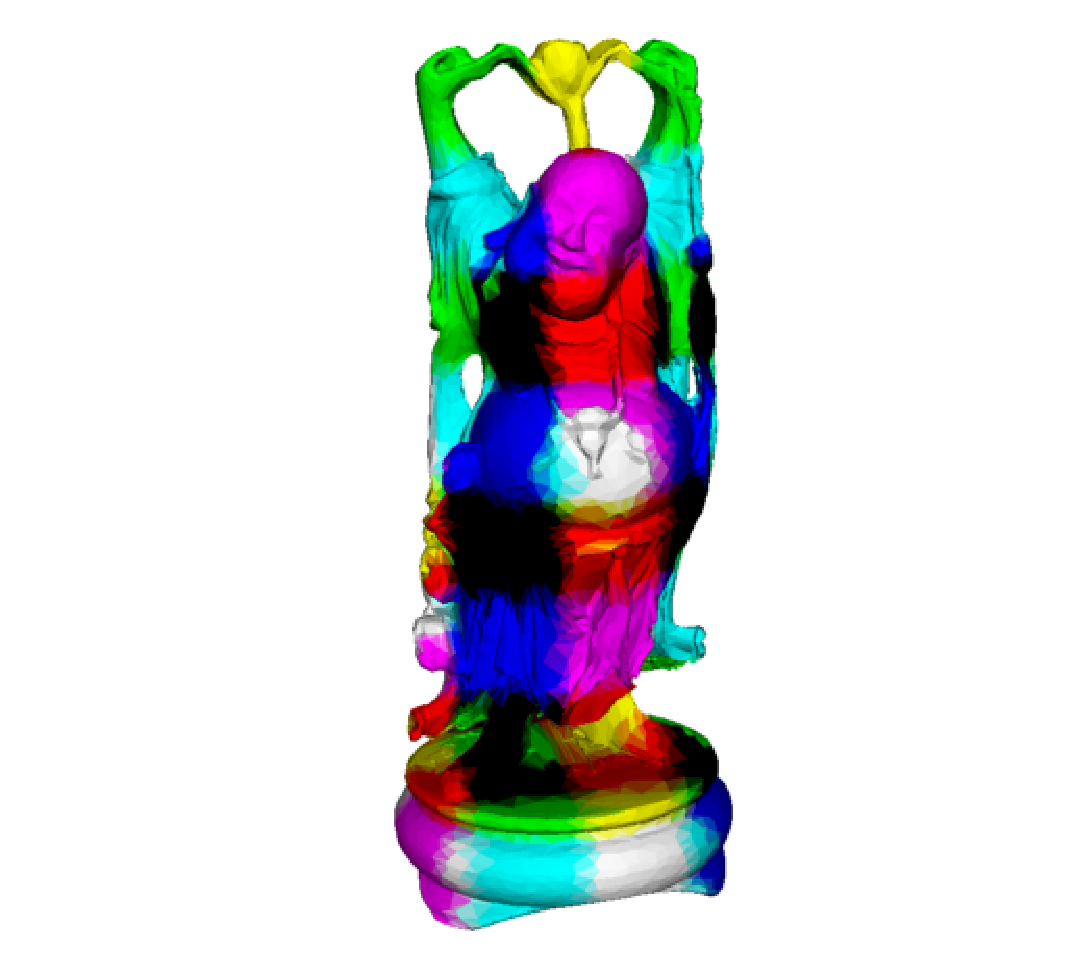
\includegraphics[scale=0.4]{buddha-checker-l025.eps}}

  \caption{Buddha}
\end{figure}

\begin{figure}
  \centering

  \subfloat[normal mapping]{
    \label{fig:dragon-normal}
    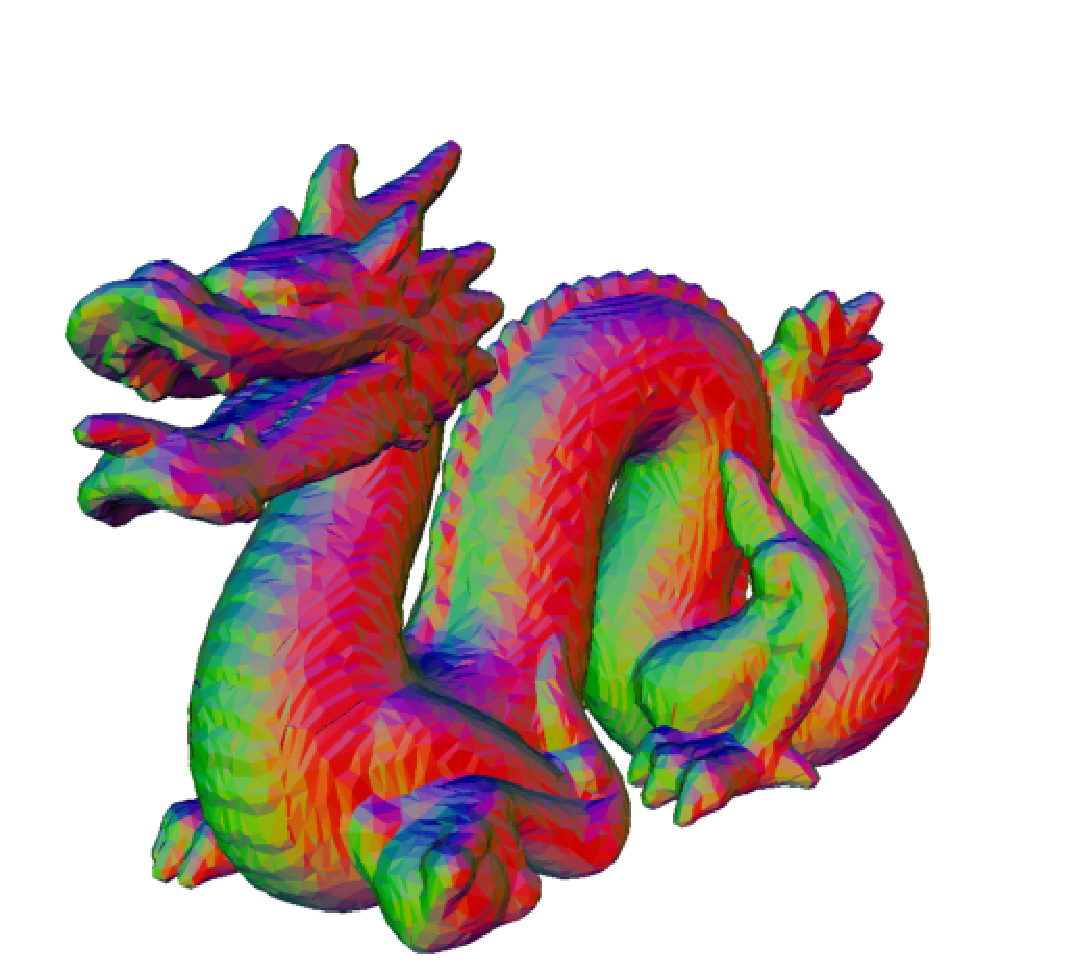
\includegraphics[scale=0.4]{dragon-normal.eps}}
  \subfloat[checker board, $L = 0.125$]{
    \label{fig:dragon-checker}
    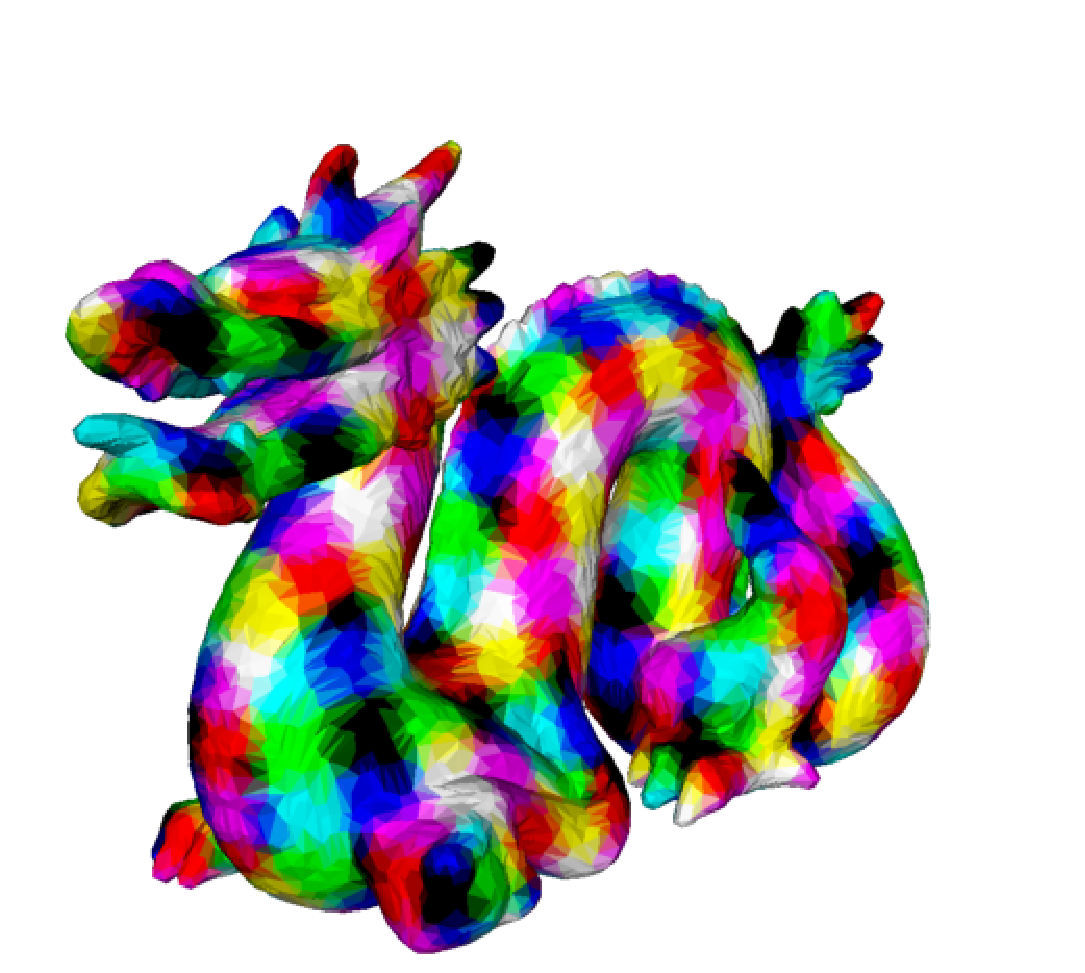
\includegraphics[scale=0.4]{dragon-checker-l0125.eps}}

  \caption{Dragon}
\end{figure}

\begin{figure}
  \centering

  \subfloat[checker board, $L = 0.5$]{
    \label{fig:icosahedron-checker1}
    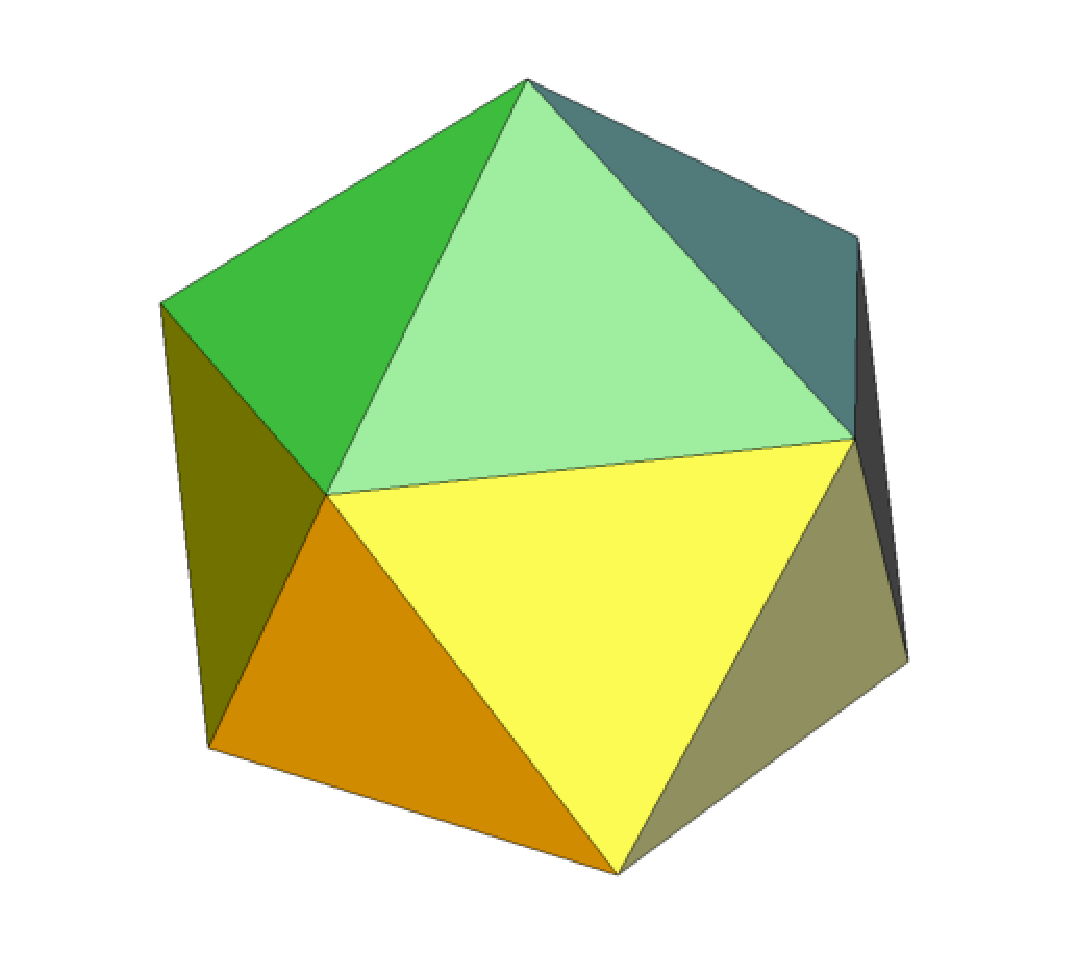
\includegraphics[scale=0.4]{icosahedron-checker-l05.eps}}
  \subfloat[checker board, $L = 1.0$]{
    \label{fig:icosahedron-checker2}
    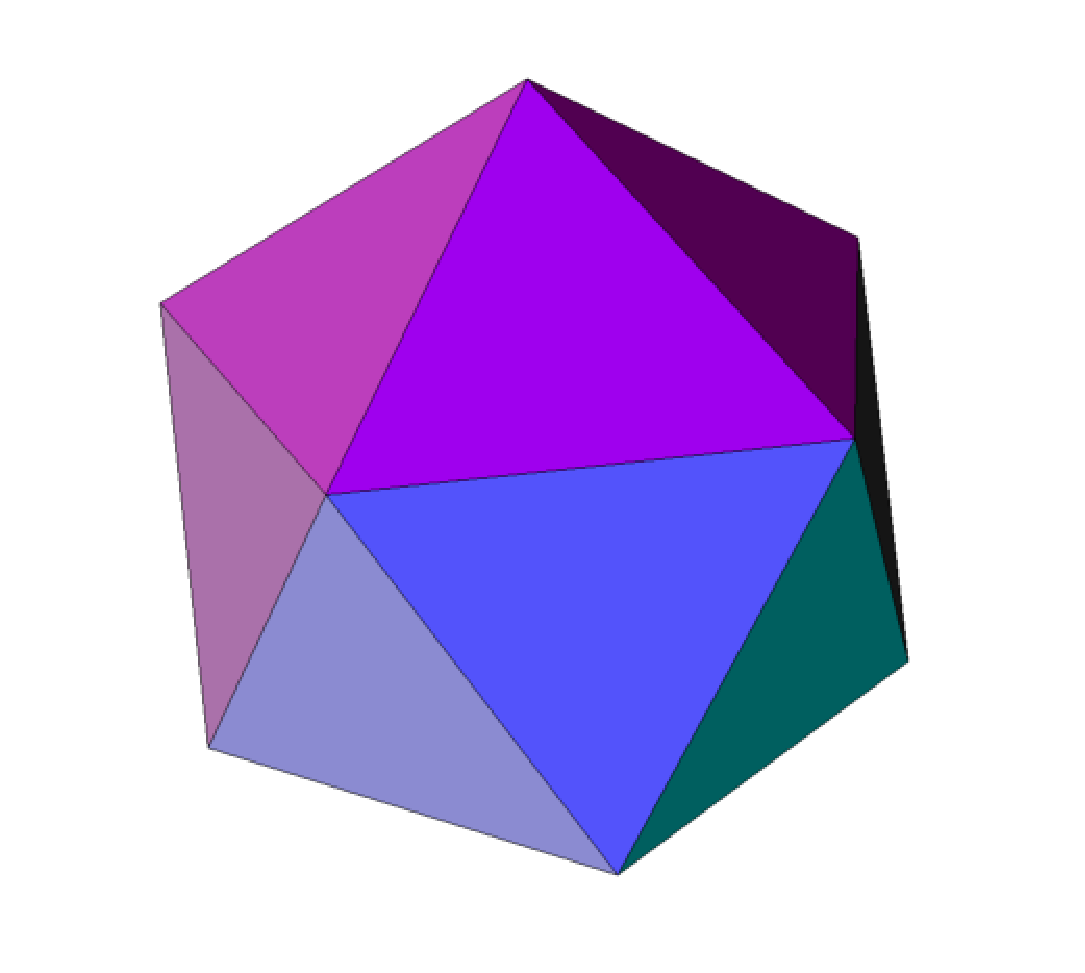
\includegraphics[scale=0.4]{icosahedron-checker-l1.eps}}

  \caption{Icosahedron}
\end{figure}

\end{document}          
